\begin{example}[Viscous Burgers 1D]
\label{ex:burgers_hest}
Based on \cite[Section 7.1.2, Example 7.5,  p. 255]{Hesthaven2008} example 7.5.
On $\Omega = \langle -1, 1 \rangle$ we will solve viscous Burgers’ equation with zero 
source function.
%\begin{equation}
%	\pdiff{u}{t} + \pdiff{}{x}\left(\frac{u^2}{2}\right) = D \pdiff{^2u}{x^2}
%\end{equation}
%where $D$ is diffusion coefficient. 
This equation has an exact solution of traveling wave 
\begin{equation}
	u_{exact} =  -\tanh\left(-\frac{2 \, t - 2 \, x - 1}{4 \,D}\right) + 1.
\end{equation}
We set boundary conditions to match the solution
\begin{equation}
	\begin{aligned}
	& u(-1, t) = -\tanh\left(-\frac{2 \, t  + 1}{4 \,D}\right) + 1, 
	&  u(-1, t) = -\tanh\left(-\frac{2 \, t - 3}{4 \,D}\right) + 1,\\
	&u_x(-1, t) = \frac{1}{2D}\tanh\left(-\frac{2 \, t + 1}{4 \, D}\right)^{2} - 
	\frac{1}{2D}, 
	&u_x(1, t) = \frac{1}{2D}\tanh\left(-\frac{2 \, t - 3}{4 \, D}\right)^{2} - 
	\frac{1}{2D}.
	\end{aligned}
\end{equation}
We will study solution at time $t = 1$ with $D = 0.001$ and $D = 0.01$. The exact 
solution is shown in \Cref{fig:burgess_hesthaven_ext}
\begin{figure}[h]
	\centering
%	\begin{tabular}{p{0.5\textwidth} p{0.5\textwidth}}
%		\vspace{0pt} 
%		\includegraphics[width=0.4\textwidth]{../figs/burgess_hesthaven_exact_t1_e001.png}
%		&
%		\vspace{0pt} 
%		\includegraphics[width=0.4\textwidth]{../figs/burgess_hesthaven_exact_t1_e01.png}
%	\end{tabular}
%	
	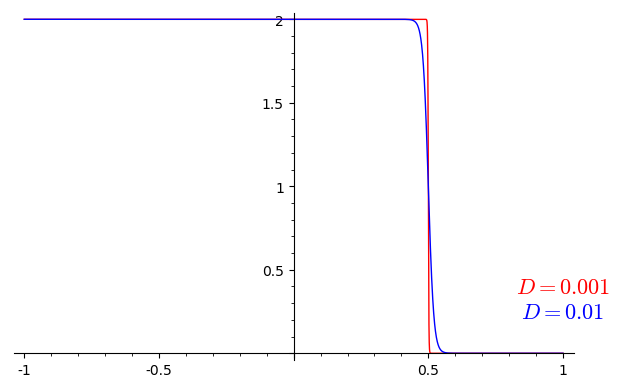
\includegraphics[scale=0.5]{../figs/burgers_hesthaven_exact_t1.png}
	\caption{\Cref{ex:burgers_hest} exact solution at $t = 1$}
	\label{fig:burgess_hesthaven_ext}
\end{figure}
Different values of coefficient $C_w$ in penalty term then different convergence 
behavior as demonstrated in \Cref{fig:burgess_ordersunlimited}. In this case increasing 
coefficient $C_w$ is detrimental to the accuracy of the solution for $D=0.001$ as it 
develops into steep step (cf. \cref{fig:burgess_hesthaven_ext}) whose approximation 
requires discontinuity in approximate solution. For $D=0.01$ the diffusion leads to much 
more gradual solution and penalty term counteracting discontinuity between elements is 
beneficial, it also helps counteract oscillations similarly to limiter in 
\Cref{ex:adv1D}. 
%Figure \ref{fig:err_sol_burges_hest} demonstrates where the errors come from.
\end{example}


\begin{figure}[h!]
	\centering
	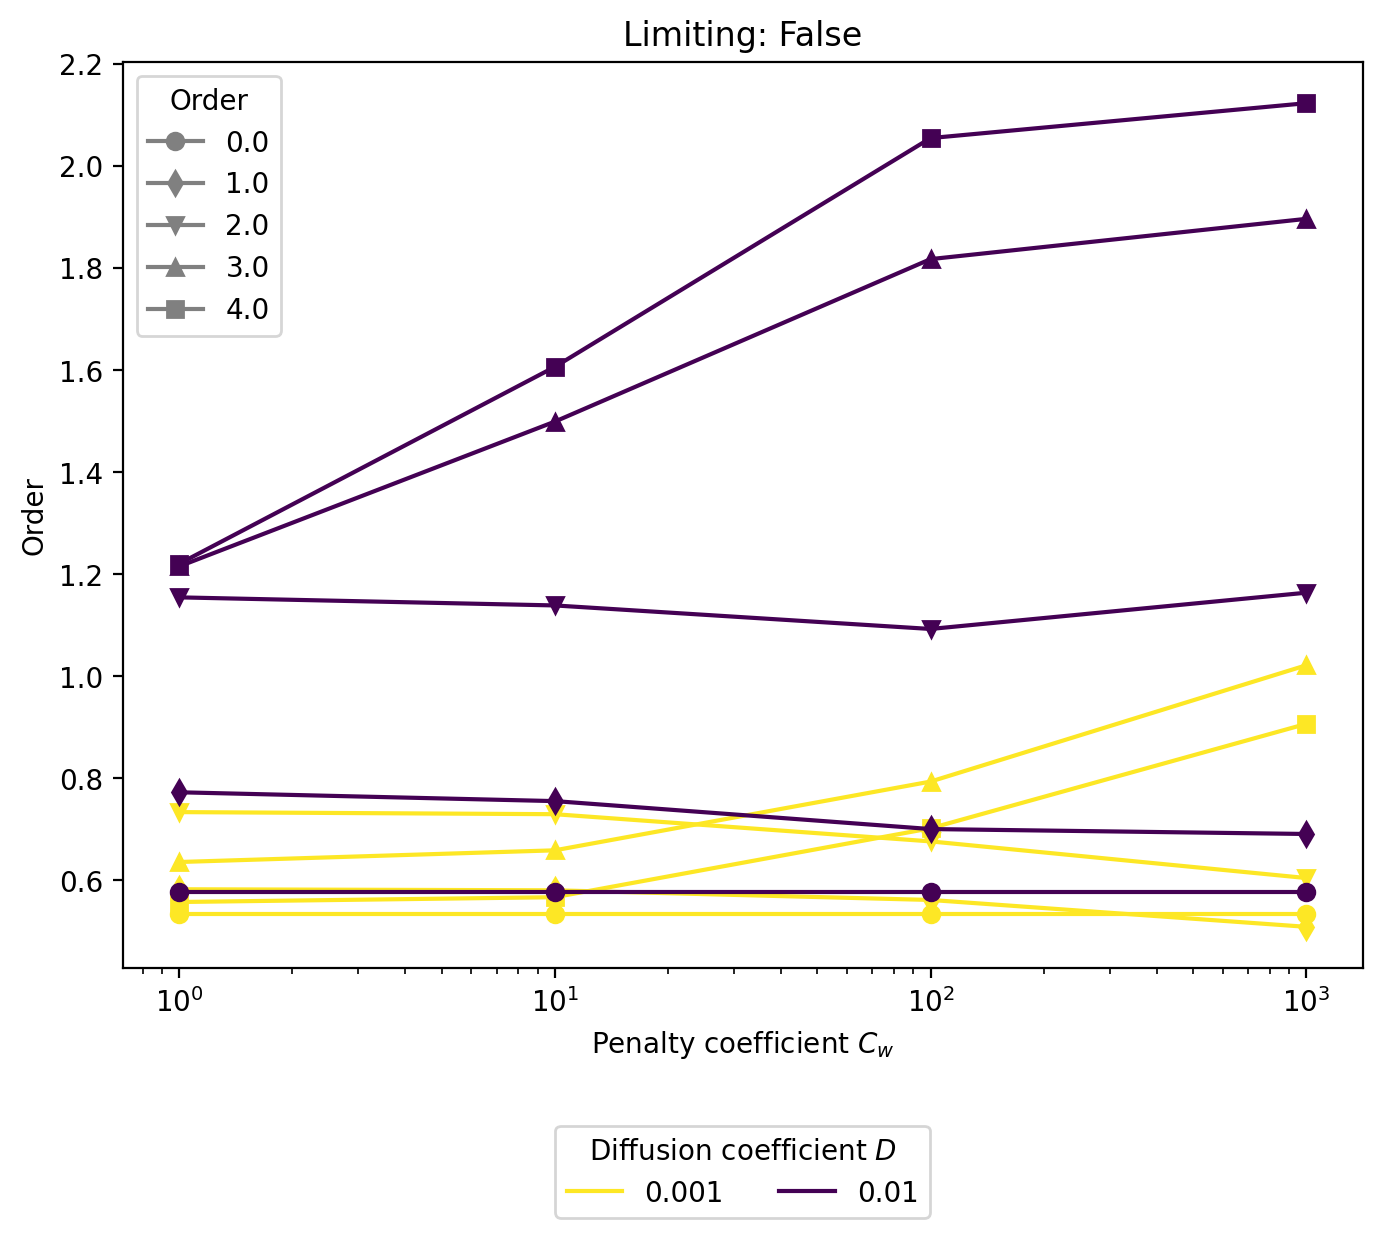
\includegraphics[scale=.6]{../figs/parametric/burgers_1D/orders_unlimited}
	\caption{\Cref{ex:burgers_hest} average order for different choice of $C_w$}
	\label{fig:burgess_ordersunlimited}
\end{figure}


\begin{figure}[p!]
	\centering
	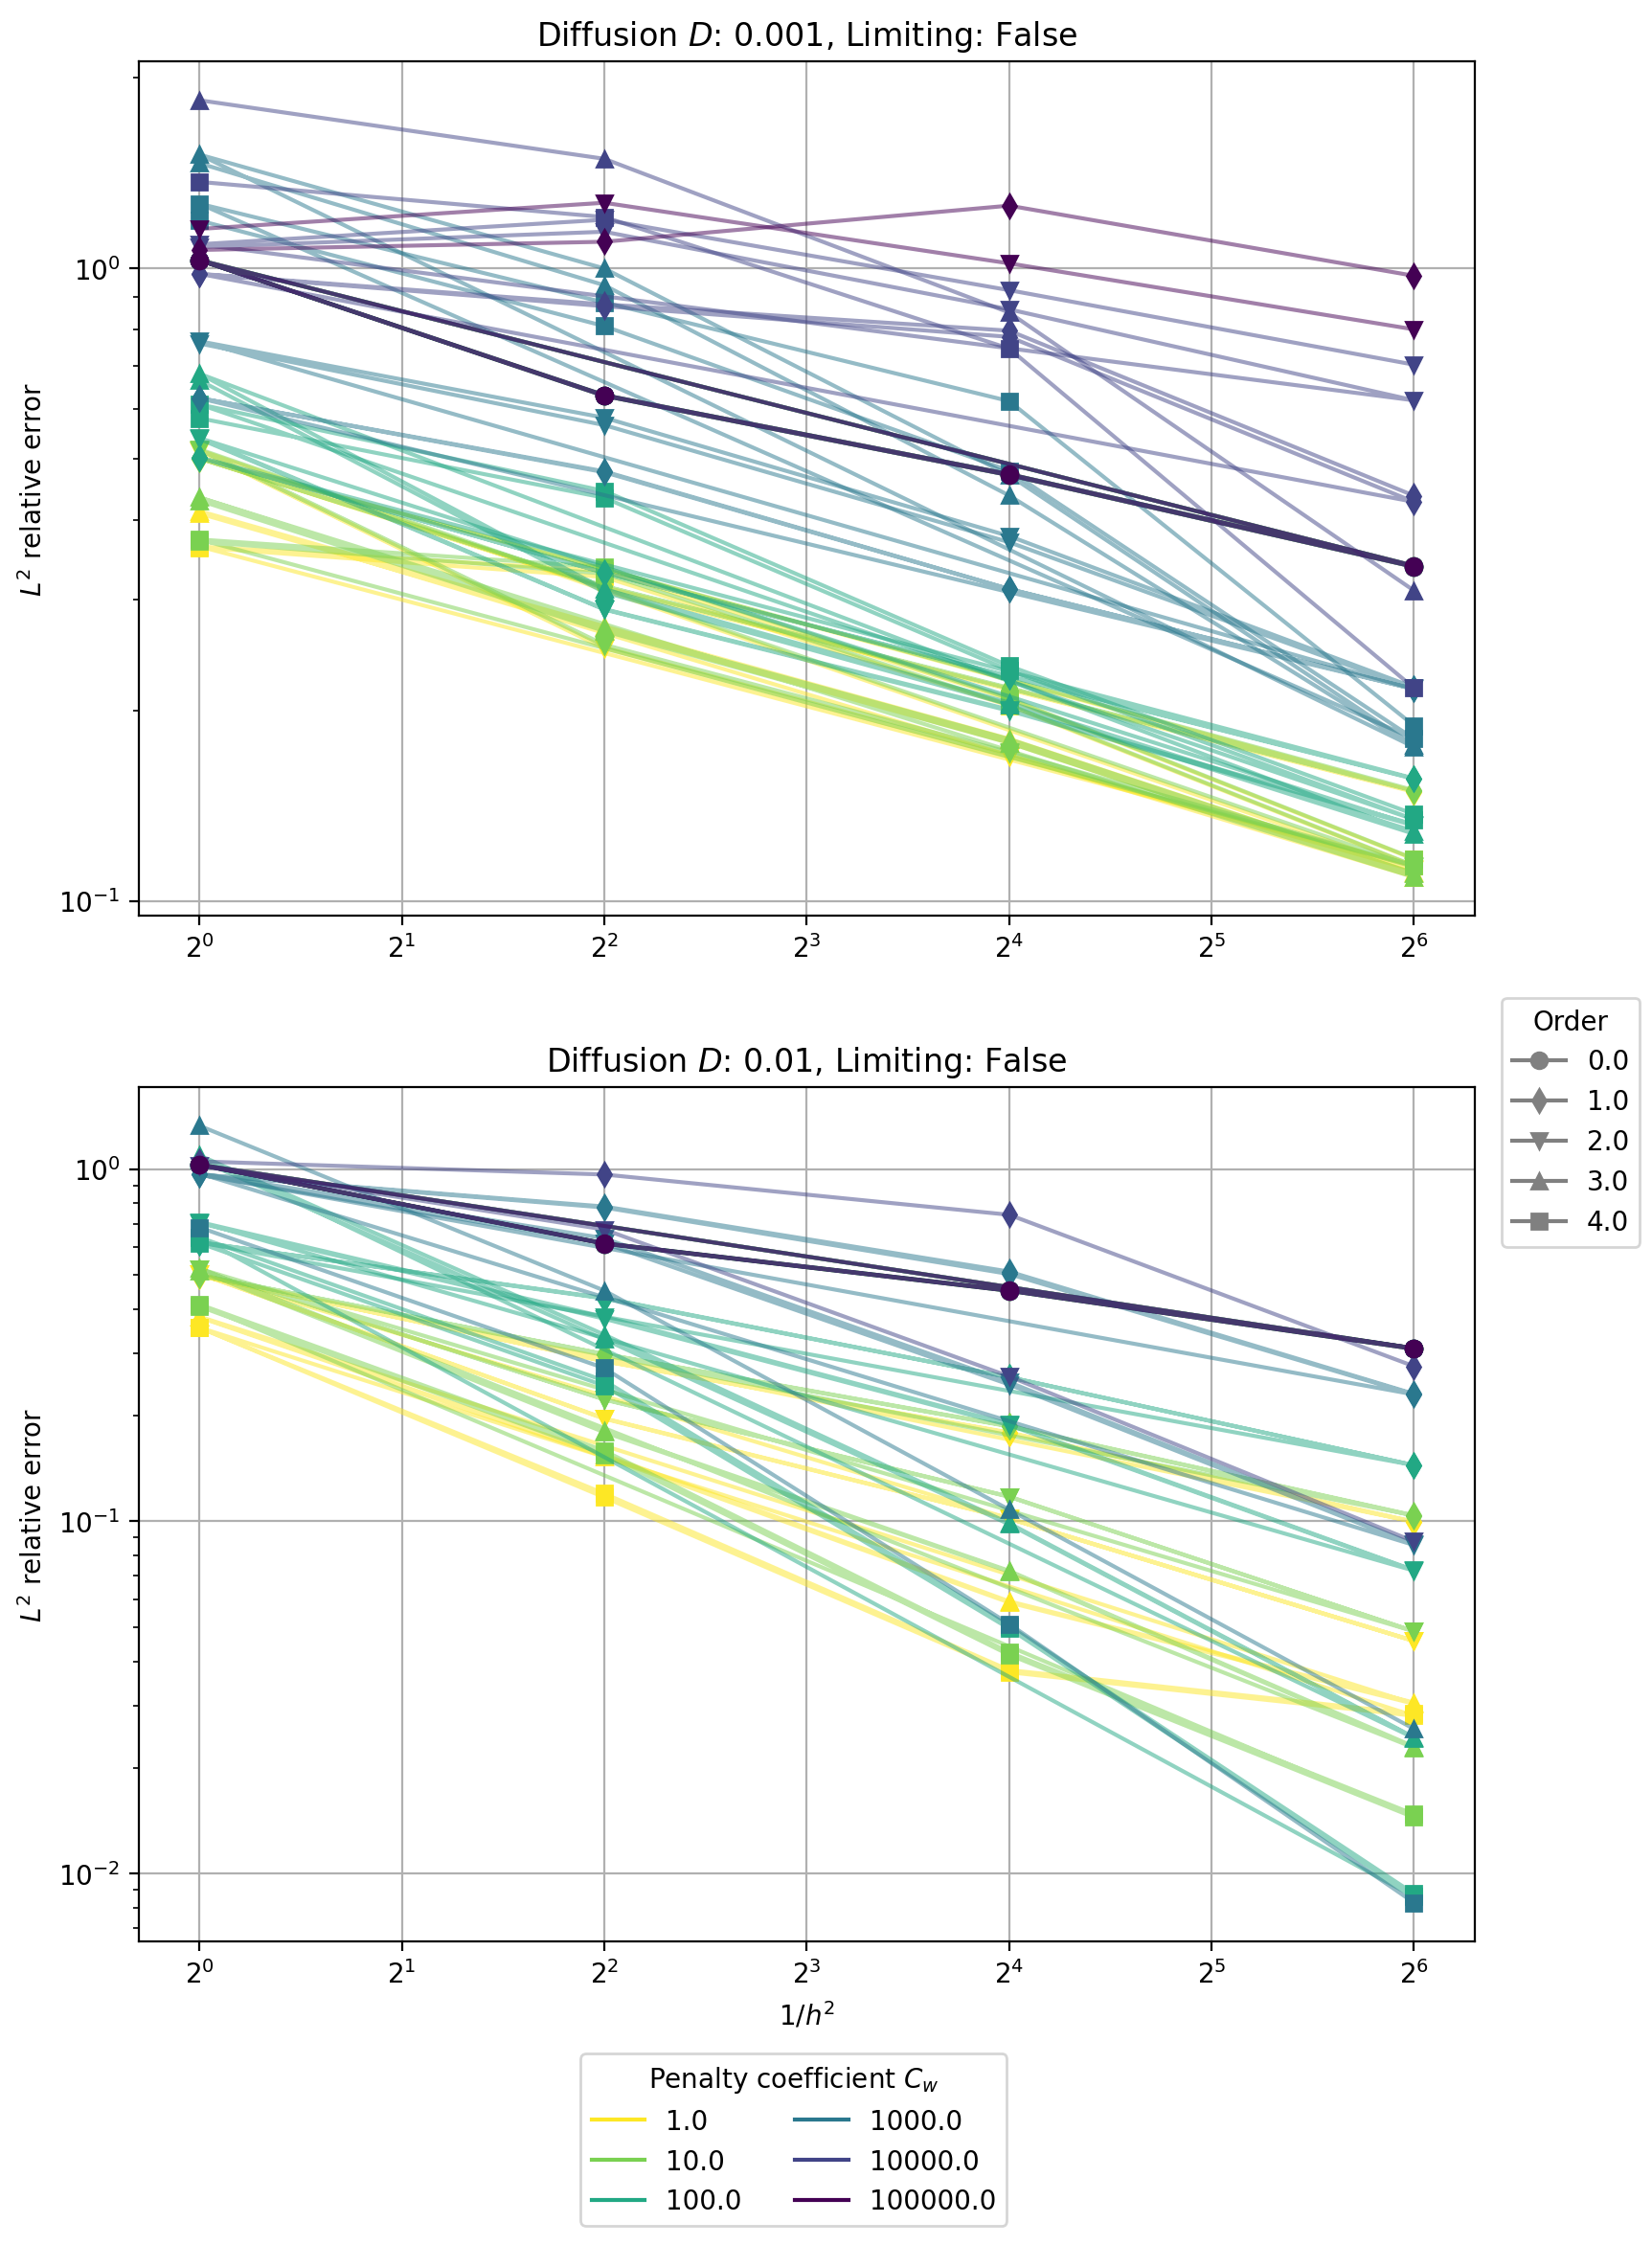
\includegraphics[width=\textwidth]{../figs/parametric/burgers_1D/_convergences_allunlimited}
	\caption{\Cref{ex:burgers_hest} convergence behavior for different choice of $C_w$}
	\label{fig:burgess_conv}
\end{figure}
\clearpage




%\begin{figure}
%	\centering
%	\includegraphics[width=\textwidth]{../figs/err-sols/burgess_hesthaven-err-sol-i20cw1_d001_t2}
%	\includegraphics[width=\textwidth]{../figs/err-sols/burgess_hesthaven-err-sol-i20cw10_d001_t2}
%	\caption{Example 9 Exact solution (gray), numerical solution (orange) and their absolute difference (red) for 
%	different orders and $h$. The left $y$ axes correspond to the solutions, the right ones to their difference.}
%	\label{fig:err_sol_burges_hest}
%\end{figure}
